\documentclass[addpoints,12pt]{exam}
\usepackage[utf8]{inputenc}
\usepackage[english]{babel}
\usepackage[letterpaper, portrait, margin=1in]{geometry}
\usepackage{amsmath}
\numberwithin{equation}{section}
\usepackage{amssymb}
\usepackage{graphicx}
\usepackage{parskip}
\usepackage{xcolor}
\usepackage{physics}
\usepackage{empheq}
\usepackage{cancel}
\usepackage{hyperref}
\hypersetup{colorlinks = true, urlcolor = blue, linkcolor = red, citecolor = red}
\usepackage{enumerate}
\usepackage{tikz}
\usepackage{float}
\usepackage{tcolorbox}
\usepackage{booktabs}
\usepackage[bottom]{footmisc}

\usepackage{xcolor}
\firstpagefooter{\color{lightgray} \today}{}{Page \thepage}
\runningfooter{\color{lightgray} \today}{}{Page \thepage}

\begin{document}
	
	\begin{center}
		\textbf{\Large{ULAB Physics \& Astronomy\\Python Module 1}}
	\end{center}
	\begin{center}
		due: TBD
	\end{center}
	
	\begin{questions}
		
		\question[10] Bash commands follow the syntax \\\verb|[command] [flags/options] [other arguments]|\\Some commands have fixed behavior and do not require any additional parameters. 
		
		However, you will often need to specify arguments. For example, \verb|cd ~/Desktop| runs the command \verb|cd| (change directory) and indicates that we would like to navigate to the desktop. 
		
		Flags are dashes followed by flag name. We use flags to indicate that a program should behave differently. Each command has it's own set of flags and options. For example, \verb|ls| with no flags lists the files in your current directory. When we include the list-all flag  \verb|ls -a| the program will list all files, including those that are normally hidden.
		
		
		For this exercise, describe the function of each of the following Bash commands. Explain what arguments you need to provide (if any). Hint: \hyperref{https://ss64.com/bash/}{}{}{https://ss64.com/bash/}
		
		\begin{parts}
			\part \verb|man|
			\part \verb|pwd| (hint: if you're confused about a directory is, read question 2)
			\part \verb|cd|
			\part \verb|ls -l|
			\part \verb|mkdir|
			\part \verb|rm| and \verb|rm -r| (hint: one is for files, one is for directories)
			\part \verb|mv|
			\part \verb|cat|
		\end{parts}
		
		Test out of these commands on the terminal! (Be careful with \verb|rm|, there is no recycle bin in Bash)
		
		\newpage
		
		\question[10] In Bash, we call folders ``directories." Directories can contain other directories or files. The root directory is the directory on your computer that contains all other directories and files. Often times, we will find the Applications, Users, etc. folders in the root directory.
		
		We can specify the path (location) of a file as an absolute path or a relative path. The absolute path is the location of a file from the root directory. The relative path is the location of a file from the current working directory (\verb|pwd|).
		
		Special symbols that stand for particular directories:
		
		``\verb|/|" root directory
		
		``\verb|.|" current working directory
		
		``\verb|..|" one directory above
		
		\begin{figure}[H]
			\centering
			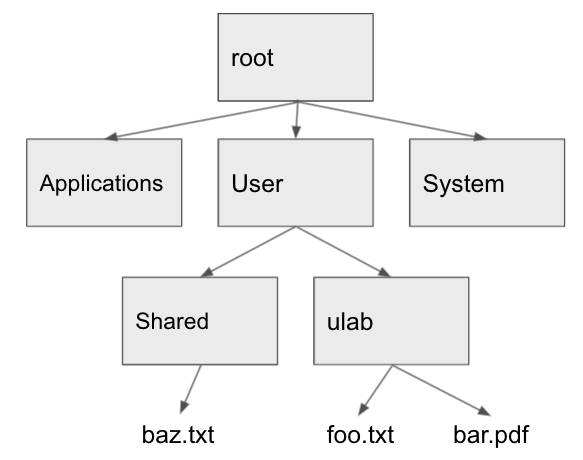
\includegraphics[width=6cm] {dir.png}
		\end{figure}
		
		For example, \verb|foo.txt| has absolute path \verb|/User/ulab/foo.txt|. If our current directory is \verb|/User/Shared|, then the relative path is \verb|../ulab/foo.txt| (make sure you understand why this is the case!)
		
		For the following exercises, the current directory is \verb|/User/Shared|.
		
		\begin{parts}
			\part What is the absolute path to the directory \verb|baz.txt|?
			
			\part What is the absolute and relative path to \verb|bar.pdf|?
			
			\part What is the relative path to \verb|/User/System|?
			
			\part The \verb|cd| command accepts both absolute and relative paths. What is the command to navigate to the ulab folder?
			
		\end{parts}

		\vspace{.5in}
		
		\question[0] Follow the instructions on the installation guide to install Anaconda. You will need this for next week!
	\end{questions}
\end{document}